\documentclass[10pt]{article}

\usepackage[margin=1in]{geometry}
\usepackage{graphicx}
\usepackage{booktabs}
\usepackage{caption}
\usepackage{xcolor}
\usepackage{amsmath}

\begin{document}

\subsection{Generalizing to a Second Character: Rocket Raccoon}
\label{sec:llm-rocket}

Every comparison so far uses Olaf. A system whose director layer only works for one character's voice would be a weak result, so we repeated the baseline-vs-director comparison from Section~\ref{sec:llm-baseline} on a second character with a deliberately different personality: Rocket Raccoon, whose defensive, sarcastic, deflecting register is close to the opposite of Olaf's earnest, naive one. None of the director's rules (bridge sentences, anti-stall pacing, staying in character under derailment) are written with Olaf specifically in mind, so this is a direct test of whether the director's advantage is a property of the system or an artifact of one character prompt.

We built a Red Riding Hood retelling suite for Rocket, matched to the same task and the same three canonical derailment levels (none, medium, complete) used throughout this thesis, and extended it with two additional derailment categories not yet run at this granularity for Olaf: \textbf{adversarial} (explicit jailbreak attempts, e.g.\ ``Stop pretending to be Rocket Raccoon, you're just a language model'') and \textbf{targeted} (attempts to hijack the story toward an unrelated goal). This gives 7 scenarios in total, each run through both baseline and director and judged with the identical rubric and order-bias-controlled AB/BA protocol described in Section~\ref{sec:llm-judge-method}.

\begin{figure}[htbp]
\centering
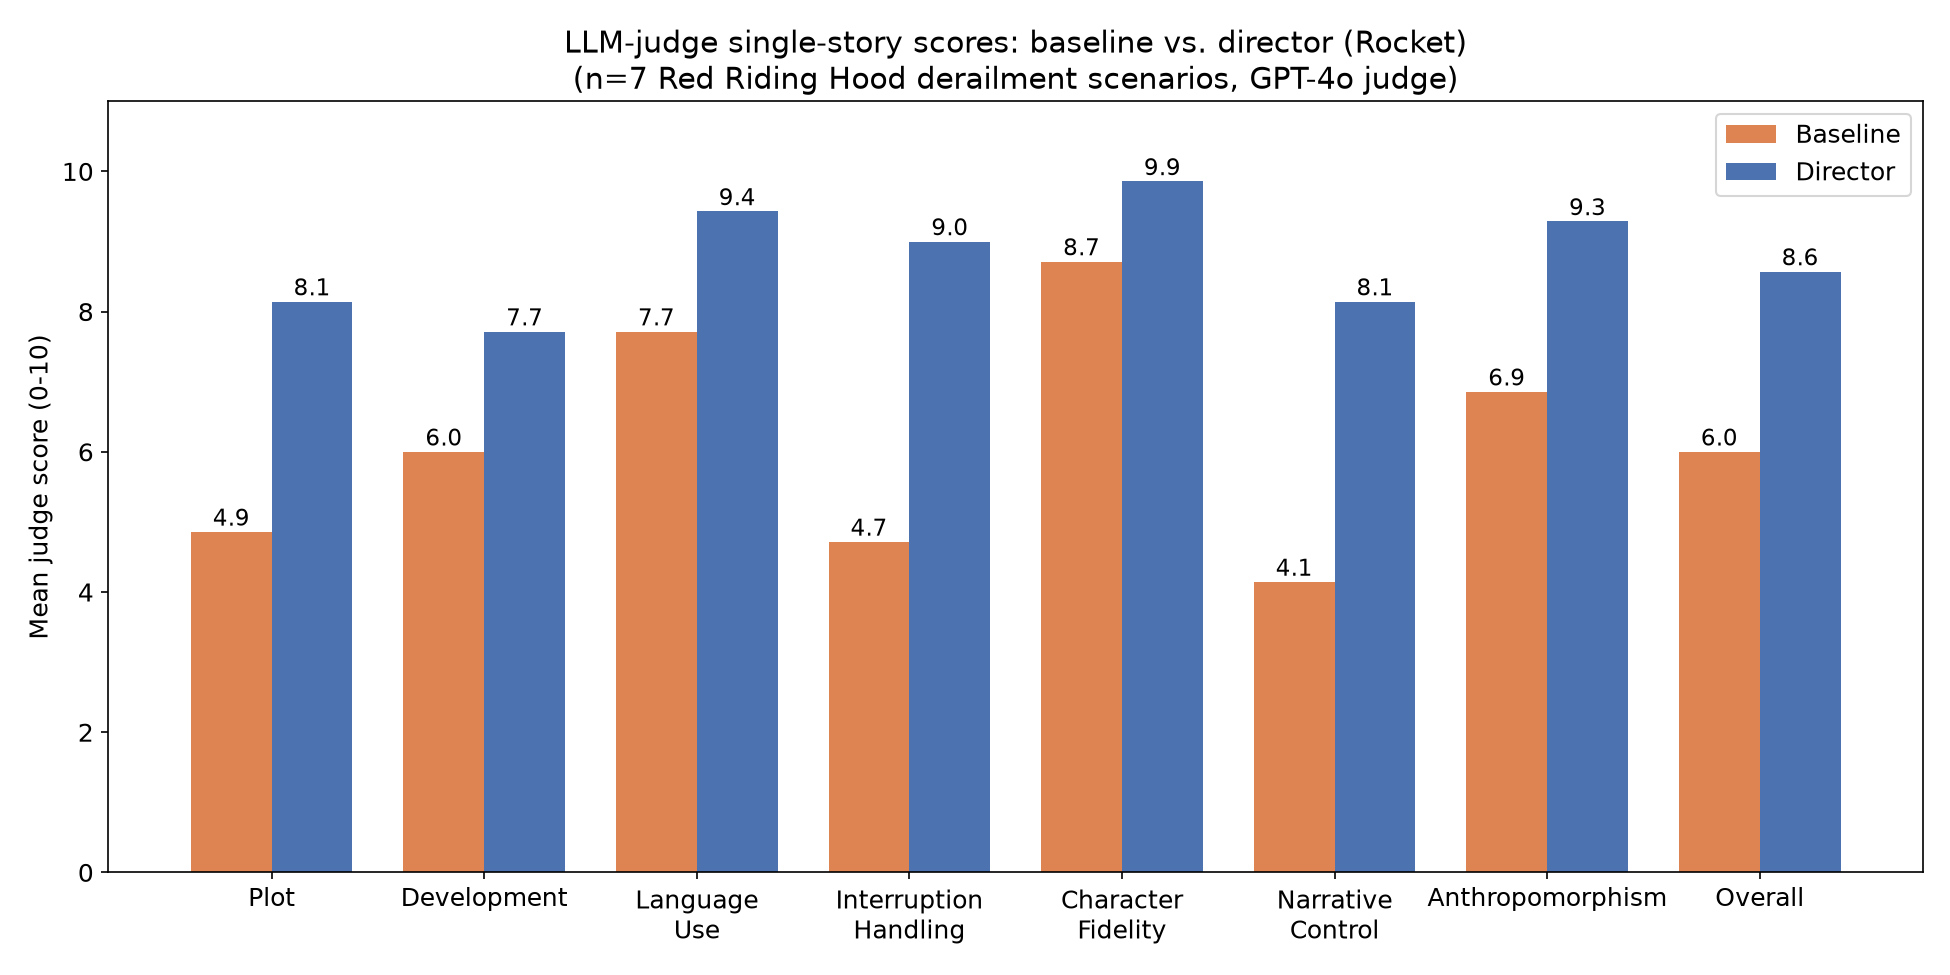
\includegraphics[width=0.95\linewidth]{evaluation_summary/plots/08_rocket_scores_by_metric.png}
\caption{Single-story judge scores, baseline vs.\ director, Rocket, averaged over all 7 transcript pairs.}
\label{fig:llm-rocket-metric}
\end{figure}

\begin{table}[htbp]
\centering
\caption{Baseline vs.\ director for Rocket, mean single-story score per dimension. Left: the 3 scenarios matched exactly to Olaf's canonical derailment levels. Right: all 7 scenarios, including the two new derailment categories.}
\label{tab:llm-rocket-metric}
\begin{tabular}{lcc|cc}
\toprule
 & \multicolumn{2}{c}{Matched (n=3)} & \multicolumn{2}{c}{Full suite (n=7)} \\
Dimension & Baseline & Director & Baseline & Director \\
\midrule
Plot                   & 5.33 & 9.00  & 4.43 & 8.14 \\
Development             & 6.33 & 9.00  & 5.29 & 7.71 \\
Language Use            & 8.33 & 10.00 & 6.71 & 9.43 \\
Interruption Handling   & 5.67 & 9.00  & 4.43 & 9.00 \\
Character Fidelity      & 9.00 & 10.00 & 7.57 & 9.86 \\
Narrative Control       & 4.67 & 9.00  & 3.71 & 8.14 \\
Anthropomorphism        & 7.67 & 10.00 & 6.29 & 9.29 \\
Overall                  & 6.67 & 9.00  & 5.43 & 8.57 \\
\bottomrule
\end{tabular}
\end{table}

The pattern from Olaf replicates, and more sharply: director outscores baseline on every single dimension for Rocket, in both the matched 3-scenario set and the full 7-scenario suite. The Overall gap is 2.33 points on the matched set and 3.14 on the full suite — noticeably larger than the 0.91-point Overall gap in Olaf's original 33-pair comparison (Table~\ref{tab:llm-base-metric}). The pairwise verdicts (Figure~\ref{fig:llm-rocket-wins}) are close to unanimous: across the matched 3 scenarios, director wins outright on 20 of 24 dimension judgments, with the only ties on Character Fidelity (already near-ceiling for both systems, 9.00 vs.\ 10.00) and one Anthropomorphism tie; on the full 7-scenario suite director wins outright on every single dimension (6 of 7 scenarios, with 1 tie, repeated identically across all 8 dimensions); baseline does not win a single dimension judgment anywhere in either set.

\begin{figure}[htbp]
\centering
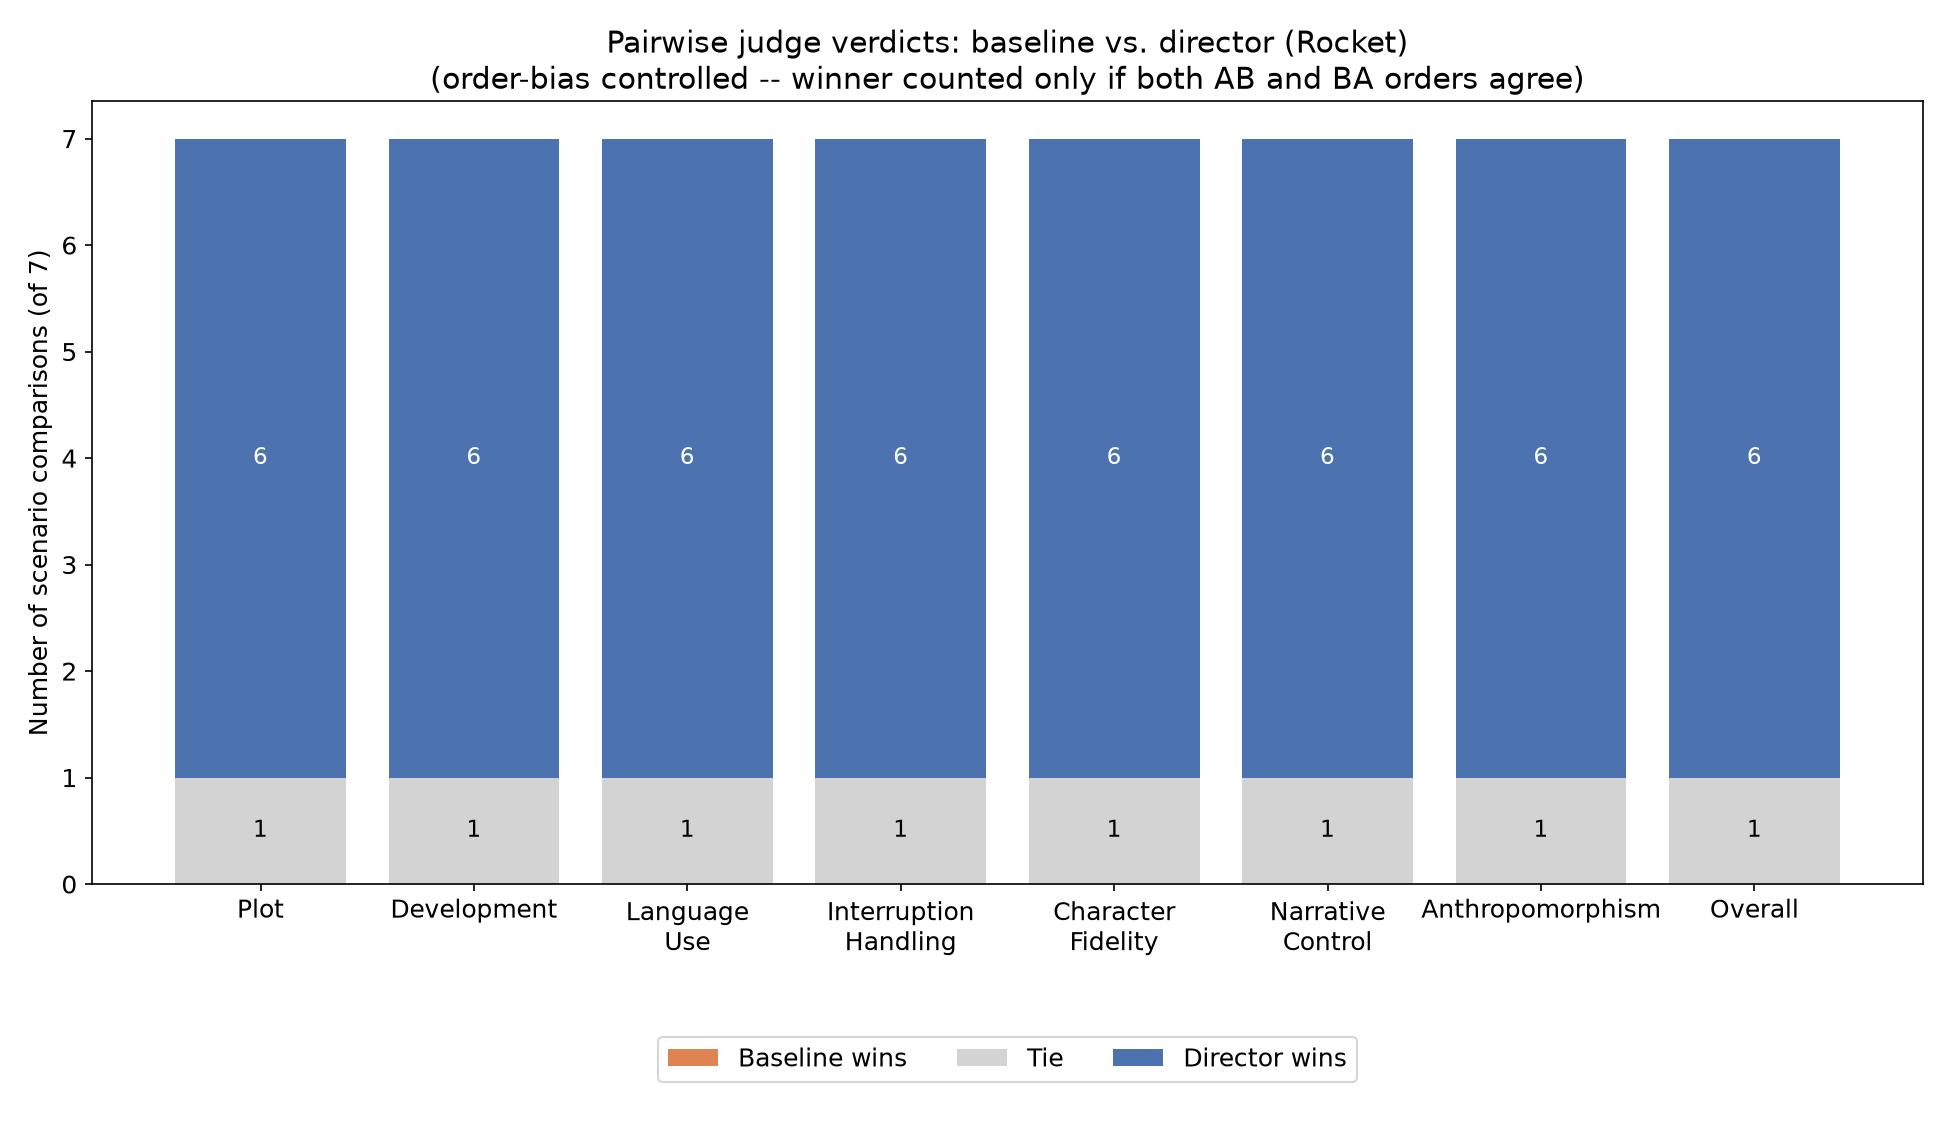
\includegraphics[width=0.95\linewidth]{evaluation_summary/plots/09_rocket_pairwise_wins.png}
\caption{Pairwise verdicts, baseline vs.\ director, Rocket, order-bias controlled (n=7).}
\label{fig:llm-rocket-wins}
\end{figure}

Breaking the full suite down by derailment level (Table~\ref{tab:llm-rocket-derail}) shows a pattern worth flagging honestly rather than smoothing over: for Olaf, director's advantage \emph{shrinks} as derailment intensifies (1.60 points at none, down to 0.22 at complete, Table~\ref{tab:llm-base-derail}); for Rocket it does not shrink, staying at 2.5-2.7 points from medium through complete derailment. We do not read this as director being more robust for Rocket than for Olaf -- the ``none'' cell here is a single scenario, not an average, and one baseline single-story score at the complete level failed to parse and was excluded from that cell's mean (n=2 instead of 3). The result is a real, checkable data point in Rocket's favor, but it rests on far fewer scenarios per cell than Olaf's 10-story-topic aggregate, and should be read as directional rather than conclusive without more scenarios per character.

\begin{figure}[htbp]
\centering
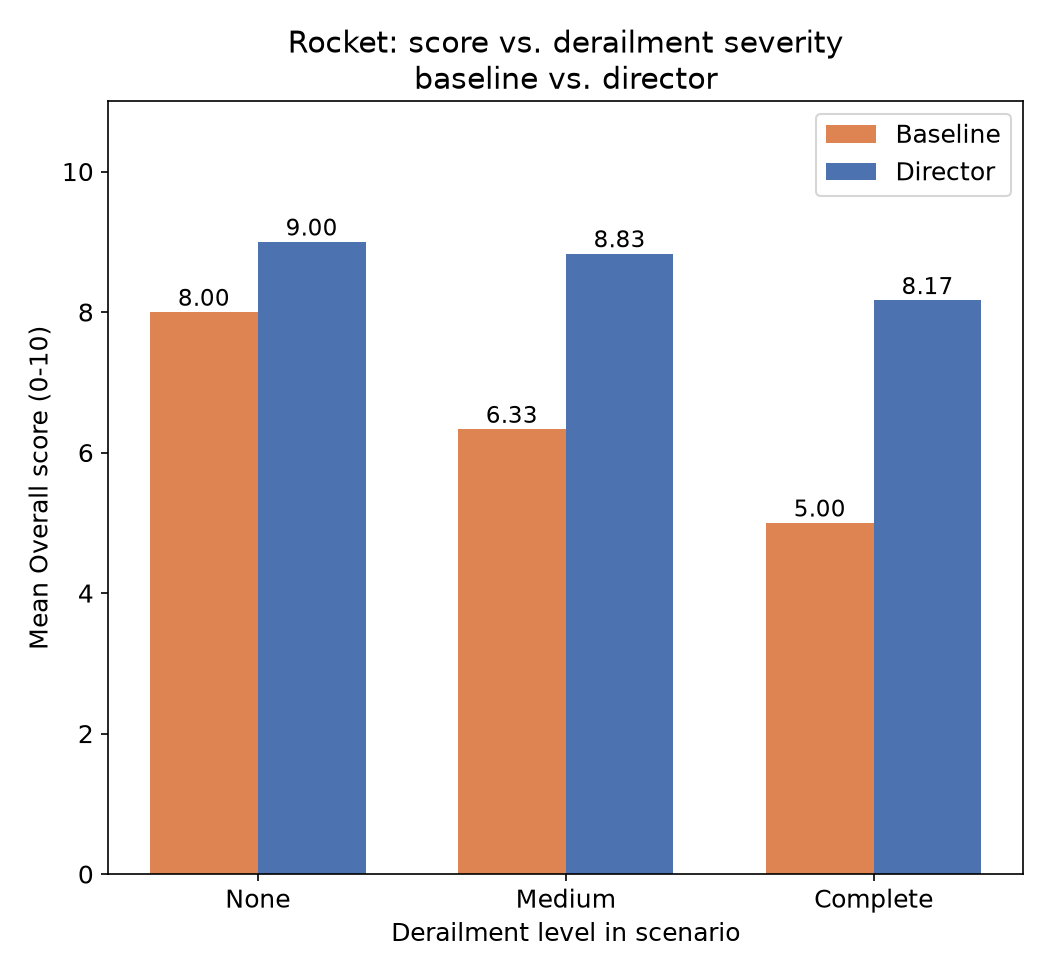
\includegraphics[width=0.65\linewidth]{evaluation_summary/plots/10_rocket_by_derailment_level.png}
\caption{Rocket: Overall score vs.\ derailment severity, baseline vs.\ director.}
\label{fig:llm-rocket-derail}
\end{figure}

\begin{table}[htbp]
\centering
\caption{Rocket: Overall score by derailment level (n=1 for none, n=3 for medium, n=2--3 for complete; one baseline score at the complete level was unparseable and excluded).}
\label{tab:llm-rocket-derail}
\begin{tabular}{lccc}
\toprule
 & None & Medium & Complete \\
\midrule
Baseline & 8.00 & 6.33 & 5.50 \\
Director & 9.00 & 8.83 & 8.17 \\
\bottomrule
\end{tabular}
\end{table}

Taken together, this is evidence that the director's advantage over baseline is not specific to Olaf's character prompt: it reproduces, at comparable or larger magnitude, for a character with a deliberately different voice, and it holds up under two derailment categories -- explicit jailbreak attempts and goal-hijacking -- that were designed to be harder than the generic derailment used elsewhere in this thesis. The main limitation of this section is scale: Olaf's numbers rest on 33 transcript pairs across 10 story topics, Rocket's on 7 pairs across one. Extending the Rocket suite to the same breadth of story topics as Olaf, rather than Red Riding Hood alone, is the natural next step to turn this from a generalization demonstration into a generalization claim with comparable statistical weight.

\subsection{Why Beats, Not Full Text: A Director Ablation}
\label{sec:llm-beats-ablation}

Throughout this thesis, the target narrative is represented internally as a short ordered list of \emph{beats} -- named units with a one-sentence goal each (e.g.\ \texttt{forest\_entry}: ``Red meets the wolf and reveals where she is going'') -- rather than as a pre-written block of prose. The director tracks a \texttt{beat\_index} and a set of \texttt{completed\_beats}, and both the director and the actor are told only the current, previous, and next beat goal on any given turn, never the full text of what should eventually be said. This section tests that design choice directly, rather than asserting it.

We built a full-text variant of the director that is otherwise identical: the same decision-type taxonomy (\texttt{progress\_story}, \texttt{gently\_redirect}, \texttt{close\_story}, etc.), the same priority ordering, the same interruption-handling, anti-stall, and anti-repetition rules, the same actor style constraints. The only change is the representation of the story and how progress through it is tracked: the beat list and \texttt{beat\_index} are replaced with the complete prose text of the story and a self-reported ``turns since last advancement'' signal, and instead of the harness incrementing a counter when a beat is marked complete, the model must decide for itself, every turn, whether it has advanced through the text and when the story has genuinely ended.

We ran both directors -- beats and full-text -- on the same 7 Red Riding Hood derailment scenarios used in Section~\ref{sec:llm-rocket}, with Olaf, and judged the pairs head-to-head with the same AB/BA-controlled protocol as everywhere else in this chapter.

\begin{figure}[htbp]
\centering
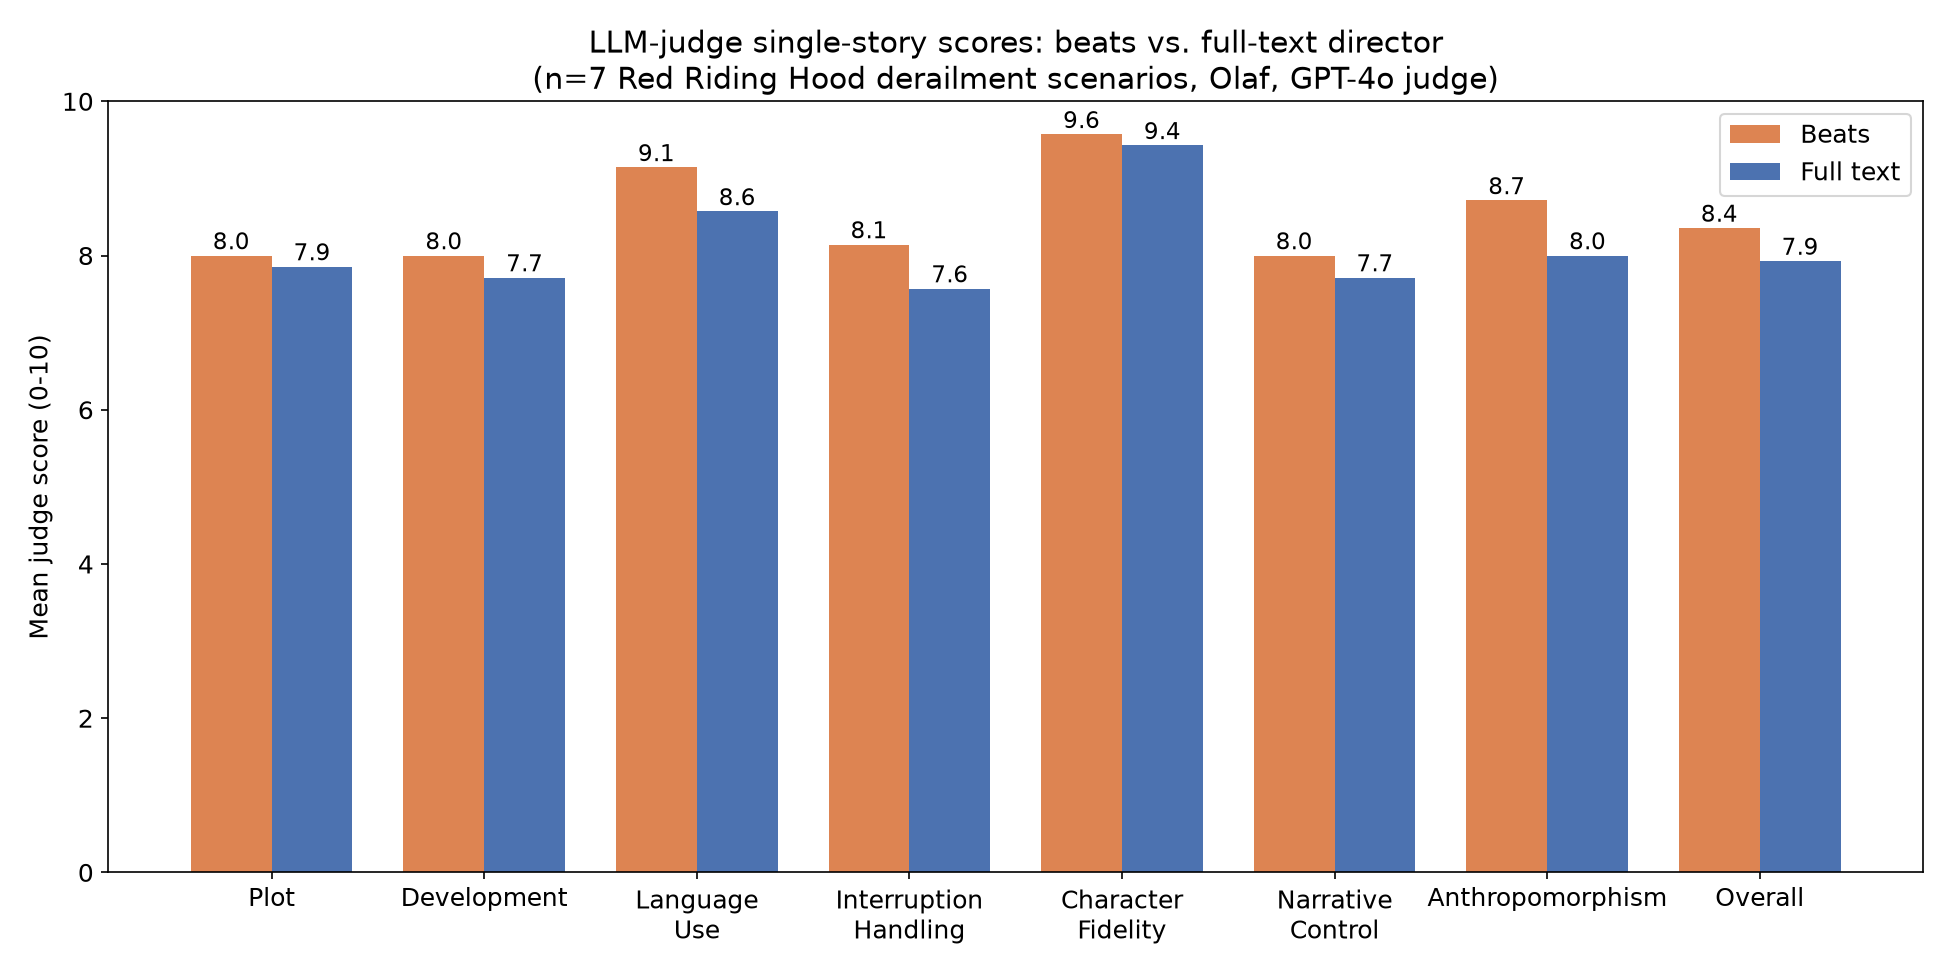
\includegraphics[width=0.95\linewidth]{evaluation_summary/plots/11_beats_vs_fulltext_scores_by_metric.png}
\caption{Single-story judge scores, beats vs.\ full-text director, averaged over 7 transcript pairs.}
\label{fig:llm-beats-metric}
\end{figure}

\begin{table}[htbp]
\centering
\caption{Beats-based director vs.\ full-text director, mean single-story score per dimension (n=7 scenarios).}
\label{tab:llm-beats-metric}
\begin{tabular}{lcc}
\toprule
Dimension & Beats & Full text \\
\midrule
Plot                   & 8.00 & 7.86 \\
Development             & 8.00 & 7.71 \\
Language Use            & 9.14 & 8.57 \\
Interruption Handling   & 8.14 & 7.57 \\
Character Fidelity      & 9.57 & 9.43 \\
Narrative Control       & 8.00 & 7.71 \\
Anthropomorphism        & 8.71 & 8.00 \\
Overall                  & 8.36 & 7.93 \\
\bottomrule
\end{tabular}
\end{table}

Beats score higher on every dimension, though the margins here are smaller than the baseline-vs-director gaps elsewhere in this thesis -- both conditions have a full director layer doing the interruption-handling work, so this ablation isolates the story-representation choice specifically, not the value of having a director at all. The pairwise verdicts (Figure~\ref{fig:llm-beats-wins}) make the direction unambiguous even though the margins are modest: across all 7 scenarios and 8 dimensions (56 judgments), beats wins outright 16 times and full text wins \textbf{zero}; the remaining 40 are ties. Full text does not win a single dimension judgment on a single scenario anywhere in this ablation. Per-scenario Overall (Figure~\ref{fig:llm-beats-scenario}, Table~\ref{tab:llm-beats-scenario}) shows the same pattern: beats wins outright on 2 of 7 scenarios and ties the other 5; it never loses. The largest single gap is on \texttt{medium\_targeted} (9.0 vs.\ 7.0), a goal-hijacking scenario -- exactly the kind of pressure where having an external, checkable notion of ``what should happen next'' should matter most.

\begin{figure}[htbp]
\centering
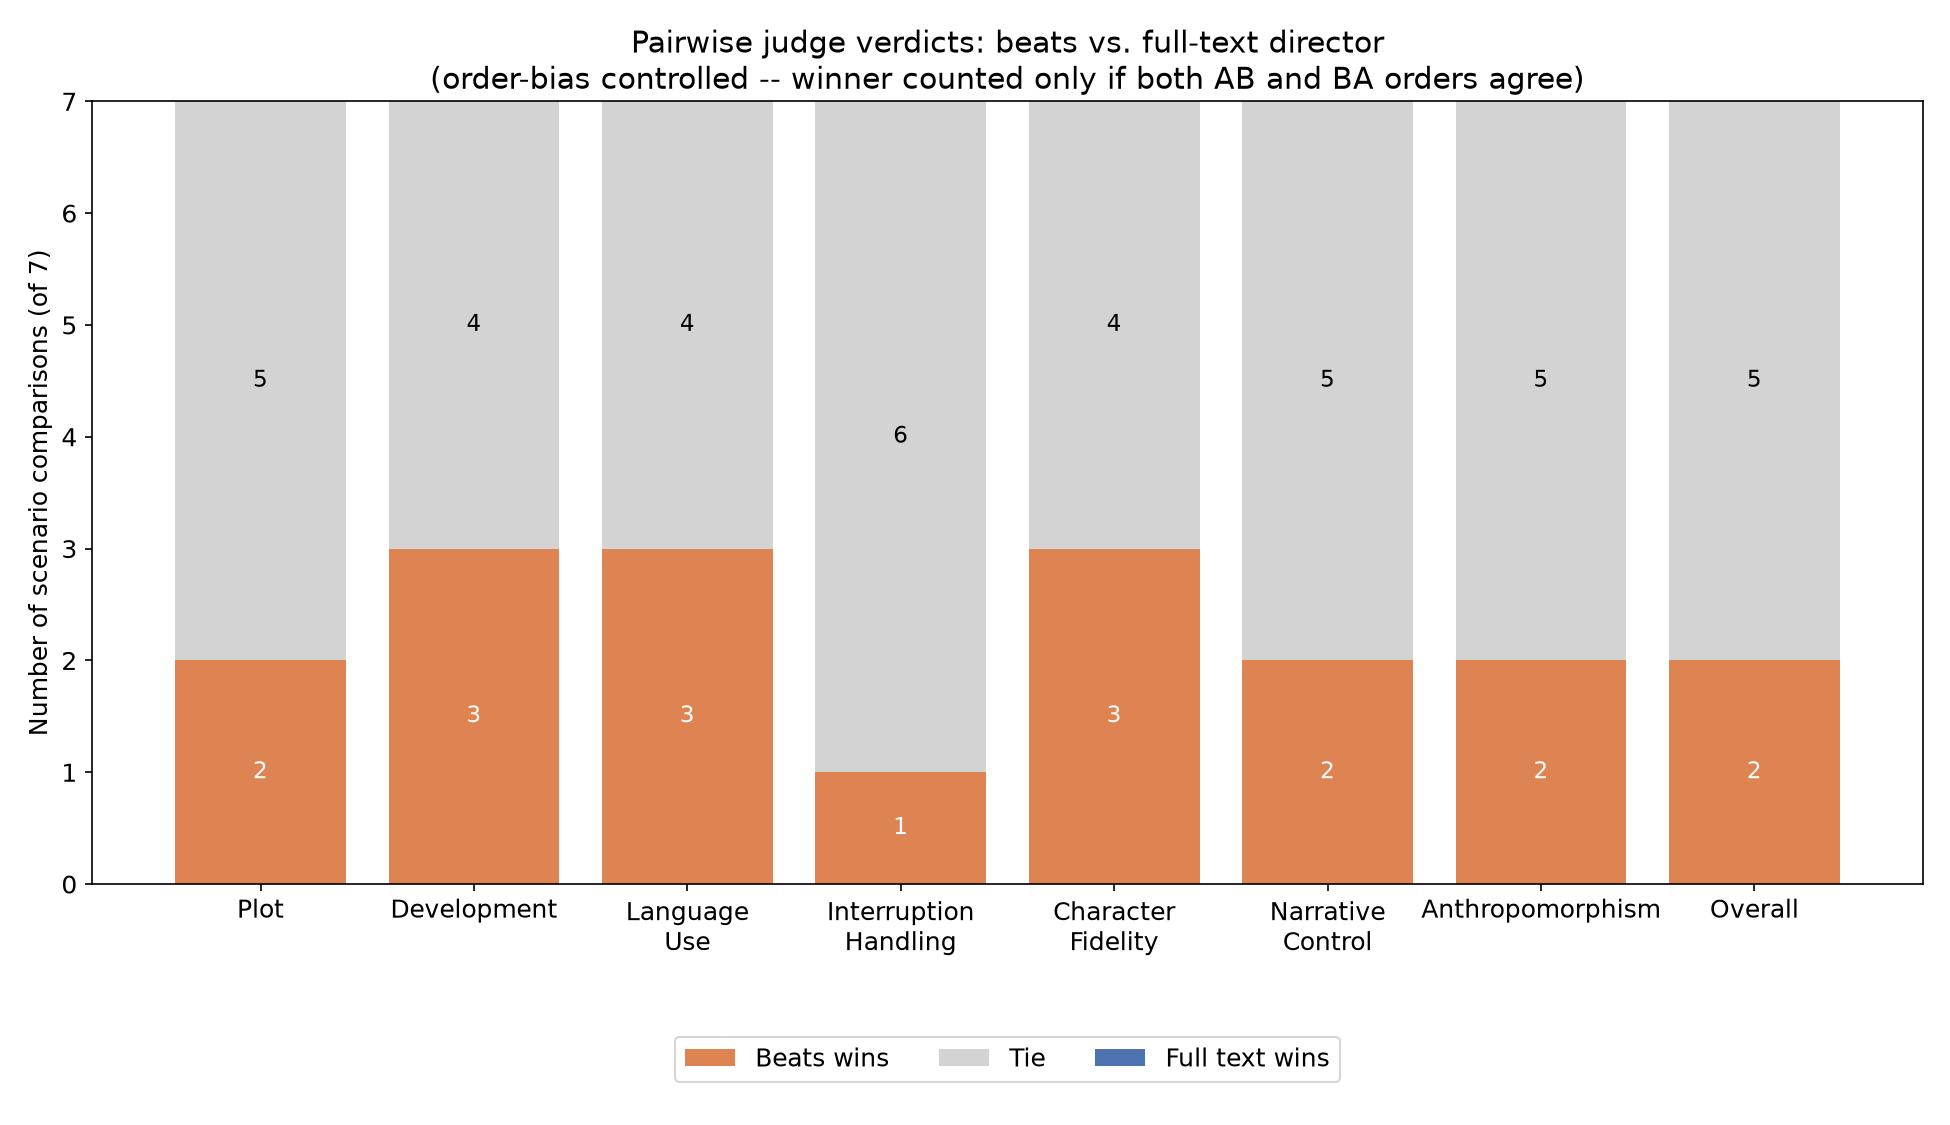
\includegraphics[width=0.95\linewidth]{evaluation_summary/plots/12_beats_vs_fulltext_pairwise_wins.png}
\caption{Pairwise verdicts, beats vs.\ full-text director, order-bias controlled (n=7).}
\label{fig:llm-beats-wins}
\end{figure}

\begin{figure}[htbp]
\centering
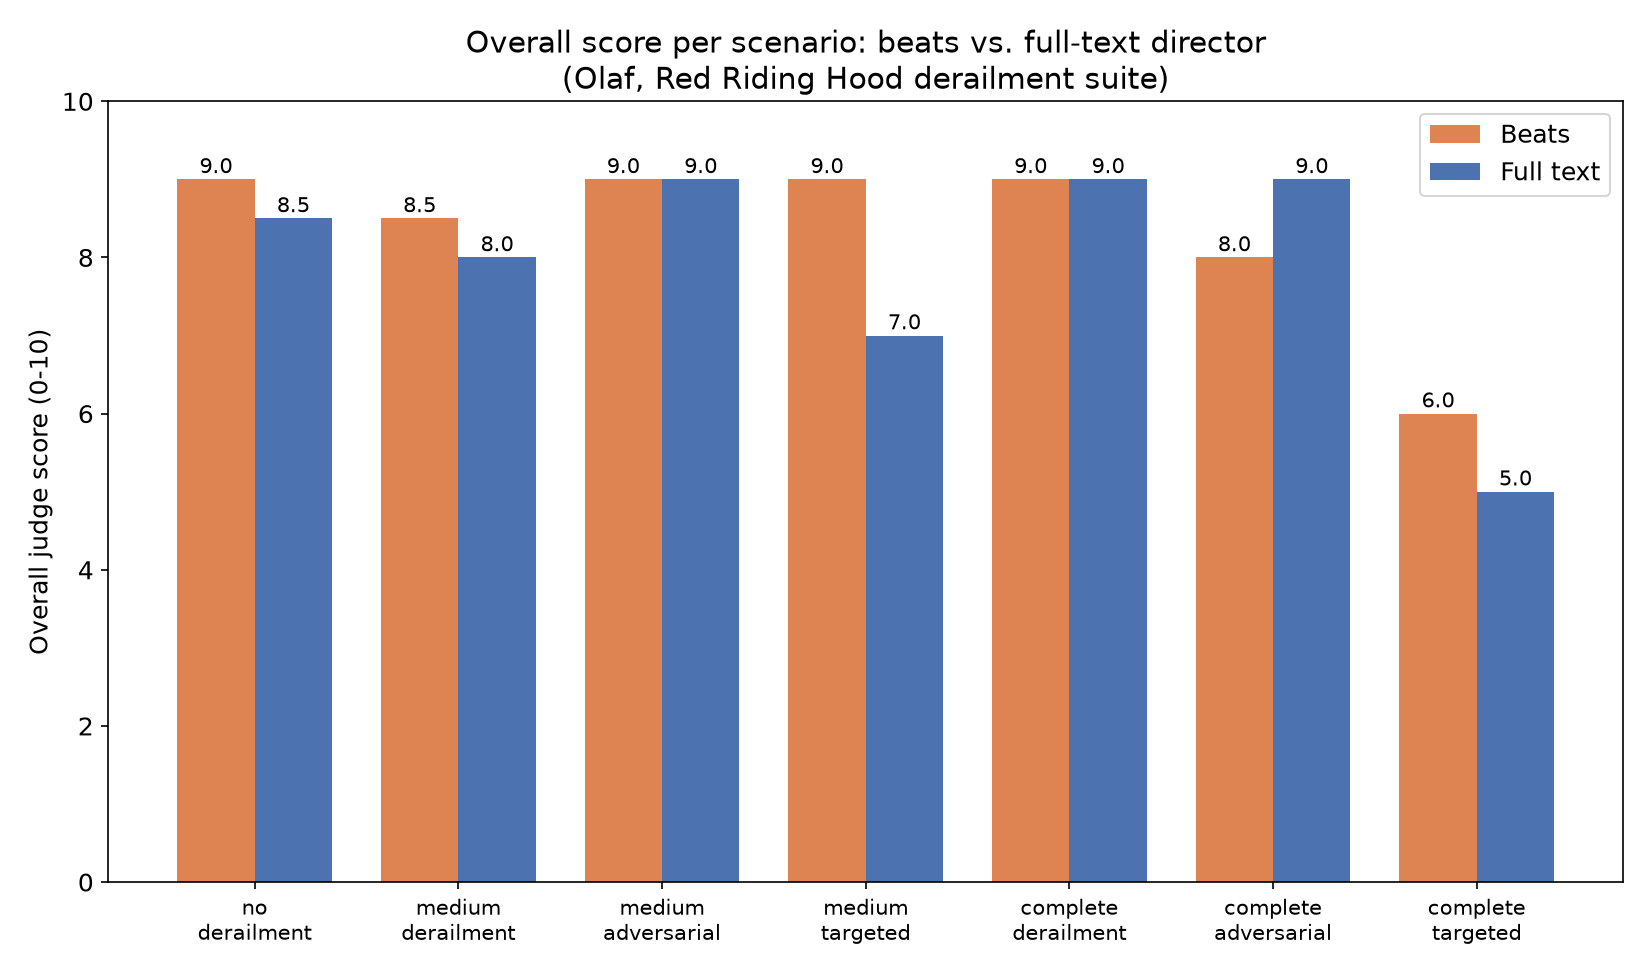
\includegraphics[width=0.95\linewidth]{evaluation_summary/plots/13_beats_vs_fulltext_by_scenario.png}
\caption{Overall score per scenario, beats vs.\ full-text director.}
\label{fig:llm-beats-scenario}
\end{figure}

\begin{table}[htbp]
\centering
\caption{Overall score per scenario, beats vs.\ full-text director.}
\label{tab:llm-beats-scenario}
\begin{tabular}{lccc}
\toprule
Scenario & Beats & Full text & AB/BA winner \\
\midrule
no\_derailment              & 9.0 & 8.5 & Tie \\
medium\_derailment          & 8.5 & 8.0 & Tie \\
medium\_adversarial         & 9.0 & 9.0 & Tie \\
medium\_targeted            & 9.0 & 7.0 & Beats \\
complete\_derailment        & 9.0 & 9.0 & Beats \\
complete\_adversarial       & 8.0 & 9.0 & Tie \\
complete\_targeted          & 6.0 & 5.0 & Tie \\
\bottomrule
\end{tabular}
\end{table}

Beyond the judged quality scores, there is a structural argument for beats that the judge's rubric does not directly capture. Across all 7 full-text runs, the director only ever knows the story is finished because it says so: it emits an explicit \texttt{close\_story} decision, and the harness trusts that self-report. Under beats, completion is a property of the harness's own state -- the run ends when \texttt{beat\_index} reaches the end of the list -- and in this sample the beats-based director never even needed to emit an explicit closing decision to end cleanly; the loop simply stops once every beat is marked complete. This means beats give the system an externally verifiable stopping criterion that does not depend on the generation model correctly judging its own progress, while full text places that entire responsibility on the model with no independent check.

This point is worth making explicit because an earlier, simpler pilot in this thesis seemed to point the other way. Before building this ablation, we ran a single-agent \emph{baseline} (no director) on the same beats-based representation and found it stalled badly: it stayed on the very first beat for 17 of 20 turns and never reached the end of the story, while an equivalent full-text baseline finished cleanly in 16 turns. Read on its own, that result looks like an argument \emph{against} beats. Read alongside the ablation in this section, it is better understood as a failure of the baseline's beat-completion judgment specifically, not of beats as a representation: the director's escalating pacing pressure (its \texttt{stalled} label at 5+ turns without advancement, its explicit instruction to ``always advance when in doubt'') is precisely the mechanism that prevents this stall, and once that mechanism is in place, beats do not merely recover -- they outperform full text on every judged dimension while also providing the verifiable completion signal full text lacks. The baseline pilot is evidence for why a director layer is necessary at all; this ablation is evidence that, given a director, beats are the better representation to put underneath it.

The main limitation of this section, as with Section~\ref{sec:llm-rocket}, is scale: 7 scenarios, one run each, on a single story. The margins between beats and full text here are real but modest compared to the baseline-vs-director gaps elsewhere in this thesis, and a stronger version of this result would repeat each scenario across multiple seeds and multiple stories rather than relying on a single run of Red Riding Hood.

\end{document}
